\documentclass[11pt]{article}

% Font tiếng việt
\usepackage{fontspec}
\usepackage[vietnamese]{babel}

% Sử dụng bảng dài có thể ngắt trang, bạn cần thêm 2 gói này vào preamble
\usepackage{longtable}
\usepackage{ragged2e}


\usepackage{graphicx}
\usepackage{amsmath, amssymb, amsfonts, bm}
\usepackage{xcolor}
\usepackage{hyperref}
\usepackage{pifont}
\newcommand{\xmark}{\ding{55}}
\newcommand{\cmark}{\ding{51}}
\usepackage{array}
\usepackage{float}

\definecolor{codehighlight}{rgb}{0.95,0.95,0.92} % Using your backcolour


\hypersetup{
    colorlinks=true,
    linkcolor=blue,
    filecolor=magenta,
    urlcolor=red,
    pdftitle={Overleaf Example},
    pdfpagemode=FullScreen,
}

\setmainfont{Times New Roman}
\setsansfont{Arial}
\setmonofont{Courier New}


% Page layout
\setlength{\topmargin}{-.5in}
\setlength{\textheight}{9.25in}
\setlength{\oddsidemargin}{0in}
\setlength{\textwidth}{6.8in}

% Title formatting
\usepackage{titling}
\setlength{\droptitle}{-10em}
\pretitle{%
    \begin{center}
    \LARGE\bfseries\textcolor{green}
    \end{center}
}
\posttitle{%
    \begin{center}
    \LARGE\bfseries\textcolor{cyan}
    \end{center}
}
\title{{UnixLinux phần 3}\\[0.5em]\textcolor{cyan}{Xử lý dữ liệu qua Command line}}
\author{Đinh Nhật Thành}
\date{}
\renewcommand{\maketitle}{}

% Fancy header/footer
\usepackage{fancyhdr}
\pagestyle{fancy}
\fancyhf{}
\renewcommand{\footrulewidth}{0.4pt}
\lhead{\bfseries AI VIETNAM}
\rhead{\bfseries aivietnam.edu.vn}
\fancyfoot[C]{\thepage}

% Section format (không đánh số section)
\usepackage{titlesec}
\titleformat{\section}
{\normalfont\Large\bfseries}
{}{0em}{}

% Listings (code block)
\usepackage{listings}
\definecolor{codegreen}{rgb}{0,0.6,0}
\definecolor{codegray}{rgb}{0.5,0.5,0.5}
\definecolor{codepurple}{rgb}{0.58,0,0.82}
\definecolor{backcolour}{rgb}{0.95,0.95,0.92}
\lstdefinestyle{mystyle}{
    backgroundcolor=\color{backcolour},
    commentstyle=\color{codegreen},
    keywordstyle=\color{magenta},
    numberstyle=\tiny\color{codegray},
    stringstyle=\color{codepurple},
    basicstyle=\ttfamily\footnotesize,
    breaklines=true,
    captionpos=b,
    keepspaces=true,
    numbers=left,
    numbersep=5pt,
    tabsize=2,
    showspaces=false,
    showstringspaces=false,
    showtabs=false
}
\lstset{style=mystyle}


% Colored boxes
\usepackage[many]{tcolorbox}
\definecolor{sub}{HTML}{cde4ff}
\newtcolorbox{boxC}{
    colback = sub,
    boxrule = 0pt,
    % Add this line to ensure proper font encoding for Vietnamese characters
    fontupper = \setmainfont{Times New Roman}\normalfont, % Or \setsansfont{Arial}\normalfont if you prefer Arial
}

% For math proofs or custom counters (tuỳ chọn nếu cần)
\usepackage{lipsum}
\newcounter{mycounter}
\newcommand\showmycounter{\stepcounter{mycounter}\themycounter}
\newcommand\showlips{\stepcounter{mycounter}\lipsum[\value{mycounter}]}

% Others
\usepackage{booktabs}
\usepackage{subcaption}
\usepackage{framed}
\usepackage{tikz}


%%%%%%%%%%%%%%%%%%%%%%%%%%%%%%%%%%%%%%%%%%%%%%%%%%%%%%%%%%%%%%%%%%%%%%%%%%%%%
%%%%%%%%%%%%%%%%%%%%%%%%%%%%%%%%%%%%%%%%%%%%%%%%%%%%%%%%%%%%%%%%%%%%%%%%%%%%%
%%%%%%%%%%%%%%%%%%%%%%%%%%%%%%%%%%%%%%%%%%%%%%%%%%%%%%%%%%%%%%%%%%%%%%%%%%%%%
\begin{document}
\maketitle

\begin{titlepage}
    \centering
    \vspace*{\fill}

    {\Huge \textbf{\thetitle} \par}
    \vspace{2em}

    {\Large \textbf{\theauthor} \par}
    \vspace{1em}

    {\large \today \par}

    \vspace*{\fill}
    \thispagestyle{fancy}
\end{titlepage}

\newpage
\tableofcontents
\thispagestyle{fancy}


%1%%%%%%%%%%%%%%%%%%%%%%%%%%%%%%%%%%%%%%%%%%%%%%%%%%%%%%%%%%%%%%%%%%%%%%%%%%%%%%%%%%%%%%%%%%%%%%%%%%%%%%%%%%%%%%%%%%%%%%%%%%%%%%%%%%%%%%%%%%%%%%%%%%%%%%%%%%%%%%%%%%%%%%%%%%%%%%%%%%%%%%%
\newpage

\renewcommand{\thesubsection}{\arabic{subsection}}
\newpage

\section{Giải thích thuật ngữ cơ bản}
\begin{longtable}{>{\RaggedRight\bfseries}p{0.25\textwidth} >{\RaggedRight\arraybackslash}p{0.7\textwidth}}
\toprule
\textbf{Thuật ngữ} & \textbf{Giải thích} \\
\midrule
\endfirsthead % Header cho trang đầu tiên của bảng

\toprule
\textbf{Thuật ngữ} & \textbf{Giải thích} \\
\midrule
\endhead % Header cho các trang tiếp theo

\bottomrule
\endfoot % Footer cho bảng

% -- Dữ liệu bảng bắt đầu từ đây --
Unix/Linux & Là các hệ điều hành mã nguồn mở, được xem là nền tảng cho nhiều công cụ phân tích dữ liệu hiện đại nhờ sự ổn định và hiệu quả cao. \\
\midrule
Shell & Một chương trình giao diện dòng lệnh, đóng vai trò trung gian giúp người dùng giao tiếp và ra lệnh cho hệ điều hành. Các loại phổ biến bao gồm \texttt{Bash}, \texttt{Zsh}, và \texttt{Fish}. \\
\midrule
Terminal & Là cửa sổ hoặc ứng dụng nơi người dùng gõ các lệnh để \texttt{Shell} thực thi. \\
\midrule
Distributions (Bản phân phối) & Là các phiên bản khác nhau của hệ điều hành Linux, được xây dựng và tùy chỉnh cho các mục đích sử dụng đa dạng. Ví dụ: \texttt{Ubuntu}, \texttt{Debian}, \texttt{CentOS}, \texttt{WSL}. \\
\midrule
API (Application Programming Interface) & có thể hiểu là "Giao diện cho BackEnd" vì nó cho phép ta gọi 1 hàm để `Thêm hoặc Xem hoặc Sửa hoặc Xóa`  từ 1 database hoặc file dữ liệu từ bất cứ đâu thông qua 1 đường link. Giả dụ bạn muốn code sử dụng cả Python lẫn Java, bạn có thể gọi và sử dụng output của 1 hàm Python trong Java như bình thường. \\
\midrule
CSV (Comma-Separated Values) & Định dạng tệp văn bản để lưu trữ dữ liệu dạng bảng, trong đó các giá trị được phân tách bằng dấu phẩy, rất phổ biến trong lưu trữ dữ liệu. \\
\midrule
JSON (JavaScript Object Notation) & Định dạng văn bản dùng để trao đổi dữ liệu có cấu trúc giống dictionary trong Python với mỗi giá trị đều có 1 cặp Key và Value, thường được các API sử dụng để trả về kết quả. \\
\midrule
Lệnh cơ bản & \texttt{cd}, \texttt{pwd}, \texttt{ls}, \texttt{mkdir}: \texttt{cd}: lệnh cơ bản để điều hướng, \texttt{pwd}: hiển thị vị trí của hiện tại, \texttt{ls}: liệt kê và tạo thư mục. \\
& \texttt{touch}, \texttt{cp}, \texttt{mv}, \texttt{rm}: Các lệnh để tạo, sao chép, di chuyển (đổi tên), và xóa tệp/thư mục. \\
\midrule
Lệnh xem và tìm kiếm dữ liệu cơ bản & \texttt{cat}, \texttt{head}, \texttt{tail}, \texttt{less}: Các lệnh dùng để xem nội dung tệp. \texttt{cat} hiển thị toàn bộ, \texttt{head}/\texttt{tail} xem phần đầu/cuối, và \texttt{less} xem theo từng trang. \\
& \texttt{find}, \texttt{grep}: Các lệnh để tìm kiếm tệp theo tiêu chí và tìm các dòng chứa một mẫu (pattern) nhất định. \\
\midrule
Lệnh xử lý dữ liệu cơ bản & \texttt{wc}, \texttt{sort}, \texttt{uniq}: \texttt{wc} là lệnh để đếm (dòng, từ, ký tự), \texttt{sort} sắp xếp dữ liệu và \texttt{uniq} để  lọc/đếm các dòng trùng lặp. \\
& \texttt{cut}, \texttt{sed}, \texttt{awk}: \texttt{cut} Công cụ mạnh mẽ để trích xuất dữ liệu theo cột, \texttt{sed} chỉnh sửa văn bản theo luồng và \texttt{awk} là lệnh nâng cao để xử lý dữ liệu có cấu trúc như bảng chứa trong file .csv hoặc database. \\
\midrule
Lệnh quản lý hệ thống thông dụng & \texttt{ps}, \texttt{top}, \texttt{kill}: Các lệnh để quản lý các tiến trình (process) đang chạy, \texttt{ps} giúp theo dõi, \texttt{top} kiểm soát và \texttt{kill} dừng các tác vụ. \\
& \texttt{chmod} là change mode dùng để thay đổi quyền truy cập , \texttt{chown} là change owner dùng để thay đổi quyền sở hữu của tệp/thư mục. \\
\midrule
\texttt{vi/vim} & Trình soạn thảo văn bản (i.e. IDE) hoạt động ngay trong terminal, giống như vscode nhưng mọi tính năng đều sử dụng thông qua terminal \\
\midrule
Biến môi trường (Environment Variable) & Các biến chứa thông tin về môi trường làm việc của shell, dùng để khai báo đường dẫn và hoạt động của các chương trình phân tích dữ liệu để dùng sau này. e.g. Biến \texttt{PATH} nói với Shell đường tìm lệnh \texttt{python} \\
\midrule
Pipe (\texttt{\textbar}) & Ký hiệu dùng để kết nối output của một lệnh với input của lệnh khác, tạo thành một chuỗi xử lý (pipeline) (giống như dây truyền sản xuất logistic).  \\
\midrule
Redirect (\texttt{\textgreater}, \texttt{\textgreater\textgreater}, \texttt{\textless}) & Các ký hiệu dùng để chuyển hướng đầu vào/đầu ra của một lệnh tới tệp thay vì màn hình. \\
\midrule
\texttt{Tham số (Parameter)} & là 1 cái tên đại diện cho giá trị đầu vào của 1 hàm, có thể coi nó là 1 variable được khai báo nhưng không chứa giá trị e.g. \texttt{def ham(tham\_so)} \\
\midrule
\texttt{Đối số (Argument)} & là giá trị được truyền vào tham số khi 1 hàm được gọi e.g. \texttt{ham(doi\_so)} \\
\midrule
\texttt{stdin}, \texttt{stdout}, \texttt{stderr} & Ba luồng dữ liệu chuẩn trong Linux: đầu vào chuẩn, đầu ra chuẩn, và đầu ra lỗi chuẩn. \\
\midrule
\texttt{xargs} & Lệnh nhận đầu vào và thực thi một lệnh khác với các đầu vào đó làm đối số i.e. arg . \\
\midrule
\texttt{jq} & Công cụ chuyên dụng để phân tích, lọc và biến đổi dữ liệu từ các tệp JSON. e.g. \texttt{jq .name data.json} lấy giá trị "name"  từ tệp JSON  \\
\midrule
\texttt{wget}, \texttt{curl} & công cụ để tải dữ liệu từ Internet, với \texttt{wget} phù hợp cho tệp lớn và \texttt{curl} linh hoạt cho API. e.g. \texttt{wget http://example.com/file.txt.} và \texttt{curl http://api.example.com} \\
\midrule
\texttt{tar}, \texttt{gzip}, \texttt{zcat} & Lệnh để đóng gói (\texttt{tar}), nén (\texttt{gzip}), và xem nội dung tệp nén (\texttt{zcat}) mà không cần giải nén hoàn toàn. \\
\end{longtable}

\section{Mở rộng phần 2: User Permission}
\begin{figure}[H]
	\centering
	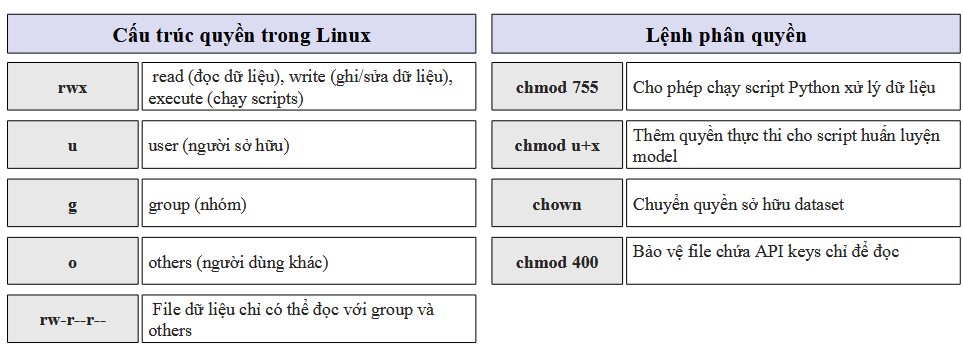
\includegraphics[width=0.8 \textwidth]{user_permission.png}
	\caption{Quyền và phân quyền files đối cho từng loại người dùng user-group-others}
	\label{fig:user_permission}
\end{figure}

\textbf{Tóm gọn hình trên, ta thấy:} \\
3 đối tượng người dùng là \texttt{u, g, o} đại diện cho \texttt{user, group, other} có vị trí mặc định là \texttt{chmod ugo} trong chmod.  Tương tự, 3 lệnh phân quyền là \texttt{r, w, e} đại diện cho \texttt{read, write, execute} cũng có vị trí mặc định là \texttt{rwx}. Nhưng nếu không muốn sử dụng cả 3 lệnh phân quyền, mình có thể dùng dấu \texttt{-} để thể hiện cho quyền rỗng, ví dụ \texttt{r-x} nghĩa là đối tượng có quyền read và execute nhưng không thể write.

\begin{itemize}
\item \texttt{rw=6} (read write), texttt{r-x=5} (read, no write permission, execite), texttt{r--=4} (only read, no write and execute), texttt{---=0} (no persmission).
\item Có thể đặt bằng số như 1 biến texttt{x=1, w=2, r=5, rwx=7} (read write execute). Với ugo là vị trí của các đối tượng trong chmod, chmod 742 ghĩa là user có quyền read write execute và group cùng others đều có quyền read. \\
\end{itemize}

\textbf{Hướng tiếp cận các câu lệnh hiệu quả:} các câu lệnh đều là các keyword viết tắt, mình có thể dễ dàng hiểu nó qua việc dịch. Ví dụ: \texttt{chmod} nghĩa là change mode, \texttt{chowner} nghĩa là change owner.

\section{Phần 3: Xử lý dữ liệu qua Command Line}
Note: giải thích lý do sử dụng -> syntax -> giải thích ngữ nghĩa sâu sau.

\subsection{Tại sao lại Xử lý dữ liệu qua Command Line (Ưu thế và bất lợi)}
\begin{itemize}
	\item \textbf{Ưu thế}: Dữ liệu được xử lý nhanh chóng vì command line loại bỏ giao diện đồ họa, giúp tiết kiệm tài nguyên và tăng tốc độ thao tác. Các lệnh có thể kết hợp linh hoạt (e.g. sử dụng chaining/piping) để xử lý dữ liệu phức tạp chỉ với một dòng lệnh. Ngoài ra, command line dễ tự động hóa bằng script, phù hợp cho xử lý dữ liệu lớn hoặc lặp đi lặp lại.
	\item \textbf{Bất lợi}: Command line có thể khó tiếp cận với người mới do cú pháp phức tạp, dễ mắc lỗi khi thao tác nhất là khi mới làm quen với Regex Express. Bạn sẽ cần phải tự viết 1 chương trình để trực quan hóa rồi chạy nó trong command line (e.g. ảnh, video) . Ngoài ra, bạn sẽ phải thực hành hằng ngày để ghi nhớ các lệnh tốt.
	\item \textbf{VSCode vs Command Line}: VSCode cung cấp giao diện đồ họa thân thiện, hỗ trợ nhiều tính năng chạy ngầm như gợi ý mã, kiểm tra lỗi, hay CoPilot và tích hợp git. Nhưng command line loại bỏ hoàn toàn những tính năng đó và chỉ tập trung vào việc xử lý chương trình. Ví dụ: VSCode có thể ngốn từ 1-3GB RAM khi chạy code vì các tính năng background trong khi Command Line chỉ cần vài trăm MB
\end{itemize}

\subsection{Regex Expression}
Regex (Regulat Expression - Biểu thức chính quy) là 1 cách \textbf{mô tả văn bản} theo một cấu trúc văn bản (text pattern) nhất định, được tích hợp trong Linux, Regex cho phép mình \textbf{tìm kiếm, thay thế hoặc phân tích các cấu trúc dữ liệu 1 cách linh hoạt} .Nếu bạn theo lập trình lâu dài, regex chắn chắn là công cụ không thể thiếu. \\ \\
Ví dụ, với regex bạn có thể tìm hoặc thay thế mọi từ có các kí hiệu 'xyz' nối sau như "helloxyz", "muaxyz", "lolxyz" hoặc thậm chí là trích xuất các hàng trong bảng theo 1 cấu trúc khi kết hợp với lệnh Linux, miễn là trích xuất thông tin có xử lý text, regex sẽ cho bạn làm điều đó hay bất kì cấu trúc nào khác phức tạp hơn 1 cách dễ dàng. \\ \\
Để tiếp cận regex 1 cách hiệu quả và vui nhất, bạn có thể bắt đầu bằng cách áp dụng các regex syntax đơn giản để truy cứu, thay thế những cấu trúc câu hoặc thực hành thêm ở \href{https://regexone.com/}{RegexOne} \\ \\

\textbf{Cách sử dụng Regex trong Command Line}: giống như 1 ngôn ngữ lập trình, regex có thể được dùng ngay trong command line, hoặc trong 1 file.

% Làm sao để compile tiếng việt trong tcolorbox hoặc codeblock
\begin{tcolorbox}[colback=backcolour, colframe=black, title=Ví dụ: Sử dụng Regex với grep]
\begin{lstlisting}[language=bash]
#!/bin/sh
# In regex, "." represents any single character. For example, "App.e" will match "Apple", "Appie", "Appae", etc., as long as it starts with "App" and ends with "e".

# Read the text file using cat
# In Linux, start the command with grep to use Regex Expression
fruits_file=`cat fruit.txt | grep App.e`

# Here, the base word (result) will be Apple,
# but since we don't know the exact spelling of Apple,
# we put a dot (.) in that position.

echo "Use '.' to find the base word, when the given word is 'App.e'"

# Display the result
echo "Result:"

echo "$fruits_file"
\end{lstlisting}
\end{tcolorbox}


\begin{itemize}
    \item \textbf{Ký tự đại diện (Wildcard Characters):}
    \begin{itemize}
        \item  \colorbox{codehighlight} {\texttt{.}} (dấu chấm): Khớp với bất kỳ ký tự nào (trừ ký tự xuống dòng). Ví dụ: {\texttt{a.b}} khớp với "axb", "ayb", "a.b".
        \item  \colorbox{codehighlight} {\texttt{*}} (dấu hoa thị): Khớp với 0 hoặc nhiều lần xuất hiện của ký tự hoặc nhóm đứng trước nó. Ví dụ: {\texttt{a*}} khớp với "", "a", "aa", "aaa". {\texttt{.*}} khtớp với bất kỳ chuỗi ký tự nào.
        \item  \colorbox{codehighlight} {\texttt{+}} (dấu cộng): Khớp với 1 hoặc nhiều lần xuất hiện của ký tự hoặc nhóm đứng trước nó. Ví dụ: {\texttt{a+}} khớp với "a", "aa", "aaa".
        \item  \colorbox{codehighlight} {\texttt{?}} (dấu hỏi): Khớp với 0 hoặc 1 lần xuất hiện của ký tự hoặc nhóm đứng trước nó (tức là tùy chọn). Ví dụ: {\texttt{colour}} khớp với "color" và "colour".
        \item \colorbox{codehighlight}{\texttt{[\^\}]*\textbackslash}} (bất kỳ kí tự nào): đại diện cho mọi Pattern, khi mình muốn truy vấn pattern \texttt{function(...)} mà không quan tâm đến bên trong có gì, ta có thể dùng  \colorbox{codehighlight}{\texttt{[\^\}]*\textbackslash}} để đại diện cho mọi pattern hay kí tự bên trong \texttt{function(...)}
    \end{itemize}

    \item \textbf{Neo (Anchors):}
    \begin{itemize}
        \item  \colorbox{codehighlight} {\texttt{\textasciicircum}} (dấu mũ): Khớp với sự bắt đầu của một dòng. Ví dụ: {\texttt{\textasciicircum Home}} khớp với "Home" chỉ khi nó ở đầu dòng.
        \item  \colorbox{codehighlight} {\texttt{\$}} (dấu đô la): Khớp với sự kết thúc của một dòng. Ví dụ: {\texttt{End\$}} khớp với "End" chỉ khi nó ở cuối dòng.
        \item  \colorbox{codehighlight} {\texttt{\textbackslash b}}: Khớp với ranh giới từ (word boundary). Ví dụ: {\texttt{\textbackslash bcat\textbackslash b}} chỉ khớp với từ "cat", không phải "category".
    \end{itemize}

    \item \textbf{Lớp ký tự (Character Classes):}
    \begin{itemize}
        \item  \colorbox{codehighlight} {\texttt{[abc]}}: Khớp với bất kỳ ký tự nào trong dấu ngoặc vuông. Ví dụ: {\texttt{[aeiou]}} khớp với bất kỳ nguyên âm nào.
        \item  \colorbox{codehighlight} {\texttt{[a-z]}}: Khớp với bất kỳ ký tự nào trong phạm vi được chỉ định. Ví dụ: {\texttt{[0-9]}} khớp với bất kỳ chữ số nào.
        \item  \colorbox{codehighlight} {\texttt{[{\textasciicircum}}abc]}: Khớp với bất kỳ ký tự nào KHÔNG nằm trong dấu ngoặc vuông. Ví dụ: {\texttt{[{\textasciicircum}0-9]}} khớp với bất kỳ ký tự nào không phải là chữ số.
        \item  \colorbox{codehighlight} {\texttt{\textbackslash d}}: Khớp với bất kỳ chữ số nào (tương đương với {\texttt{[0-9]}}).
        \item  \colorbox{codehighlight} {\texttt{\textbackslash D}}: Khớp với bất kỳ ký tự nào không phải chữ số (tương đương với {\texttt{[{\textasciicircum}0-9]}}).
        \item  \colorbox{codehighlight} {\texttt{\textbackslash w}}: Khớp với bất kỳ ký tự chữ-số hoặc dấu gạch dưới (tương đương với {\texttt{[a-zA-Z0-9\_]}}).
        \item  \colorbox{codehighlight} {\texttt{\textbackslash W}}: Khớp với bất kỳ ký tự nào không phải chữ-số hoặc dấu gạch dưới.
        \item  \colorbox{codehighlight} {\texttt{\textbackslash s}}: Khớp với bất kỳ ký tự khoảng trắng nào (space, tab, newline, v.v.).
        \item  \colorbox{codehighlight} {\texttt{\textbackslash S}}: Khớp với bất kỳ ký tự nào không phải khoảng trắng.
    \end{itemize}

    \item \textbf{Nhóm (Groups) và Tham chiếu ngược (Backreferences):}
    \begin{itemize}
        \item  \colorbox{codehighlight} {\texttt{(pattern)}}: Tạo một nhóm chụp (capturing group) cho một phần của biểu thức. Ví dụ: {\texttt{(abc)+}} khớp với "abc", "abcabc".
        \item  \colorbox{codehighlight} {\texttt{\textbackslash n}}: Tham chiếu ngược đến nội dung đã được nhóm chụp thứ \texttt{n}. Ví dụ: {\texttt{(\textbackslash w+)\textbackslash s+\textbackslash 1}} khớp với các từ lặp lại như "hello hello".
    \end{itemize}

    \item \textbf{Lượng tử (Quantifiers):}
    \begin{itemize}
        \item  \colorbox{codehighlight} {\texttt{\{n\}}}: Khớp chính xác \texttt{n} lần. Ví dụ: {\texttt{a\{3\}}} khớp với "aaa".
        \item  \colorbox{codehighlight} {\texttt{\{n,\}}}: Khớp ít nhất \texttt{n} lần. Ví dụ: {\texttt{a\{2,\}}} khớp với "aa", "aaa", v.v.
        \item  \colorbox{codehighlight} {\texttt{\{n,m\}}}: Khớp ít nhất \texttt{n} lần và nhiều nhất \texttt{m} lần. Ví dụ: {\texttt{a\{1,3\}}} khớp với "a", "aa", "aaa".
    \end{itemize}

    \item \textbf{Ký tự thoát (Escaping Characters):}
    \begin{itemize}
        \item  \colorbox{codehighlight} {\texttt{\textbackslash}}: Ký tự gạch chéo ngược dùng để thoát các ký tự có ý nghĩa đặc biệt trong Regex, biến chúng thành ký tự nghĩa đen. Ví dụ: {\texttt{\textbackslash.}} khớp với dấu chấm nghĩa đen, không phải bất kỳ ký tự nào.
    \end{itemize}
\end{itemize}

\vspace{4in} % break line using inches. 1 inch ~ 2.54 cm
\subsection{Pipe và Redirect}
Trong 4 khối lệnh, \textbf{Pipe} \texttt{(|)} và \textbf{Redirect} \texttt{(>, >>, <)} là hai công cụ rất quan trọng trong Unix/Linux, cho phép bạn nối các lệnh lại với nhau và điều khiển luồng dữ liệu đầu vào/đầu ra.
\begin{figure}[H]
	\centering
	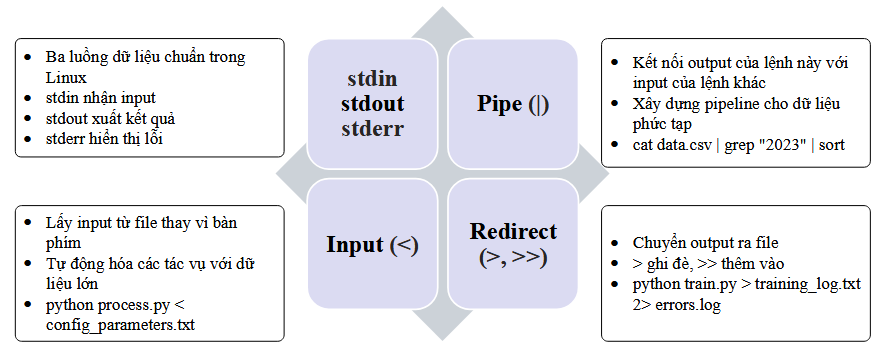
\includegraphics[width=1 \textwidth]{pipeline_redirect.png}
	\caption{4 khối lệnh cơ bản để xây dựng pipeline xử lý dữ liệu}
	\label{fig:pipeline_redirect}
\end{figure}

\vspace{6.4in} % break line using inches. 1 inch ~ 2.54 cm

\subsubsection{Minh họa flow hoạt động của Pipe và Redirect}
Lệnh Pipe lấy trong từ pipeline, trong thực tế 1 đường ống lớn là sự kết hợp của các đường ống nhỏ gồm có đầu vào và đầu ra nối lại với nhau. Tương tự như thế, Pipe có thể hiểu là các đường ống (pipelines) hay 1 hàm gồm input và output được nối lại với nhau tạo thành 1 pipe hoàn chỉnh. \\ \\

Trong hình minh họa, ta có hàm \texttt{wc -l *.pdb} dùng để đếm số dòng trong mỗi file, trong đó:
\begin{itemize}
	\item \texttt{wc} nghĩa là word count.
	\item \texttt{-l} nghĩa là list dùng đẻ liệt kê.
	\item \texttt{*.pdb} có * nghĩa là tất cả, \texttt{*.pdb} nghĩa là cho mọi file có đuôi \texttt{.pbd}.
\end{itemize}
Nếu không làm gì, output của hàm sẽ được tự động viết ra Shell, giống như trong ngôn ngữ C, mình có thể dùng mũi tên để điều chỉnh hướng của dữ liệu là ghi đè (append) output vào file (note: < để lấy input, > để ghi đè, >> để thêm vào). \\ \\

\begin{figure}[H]
	\centering
	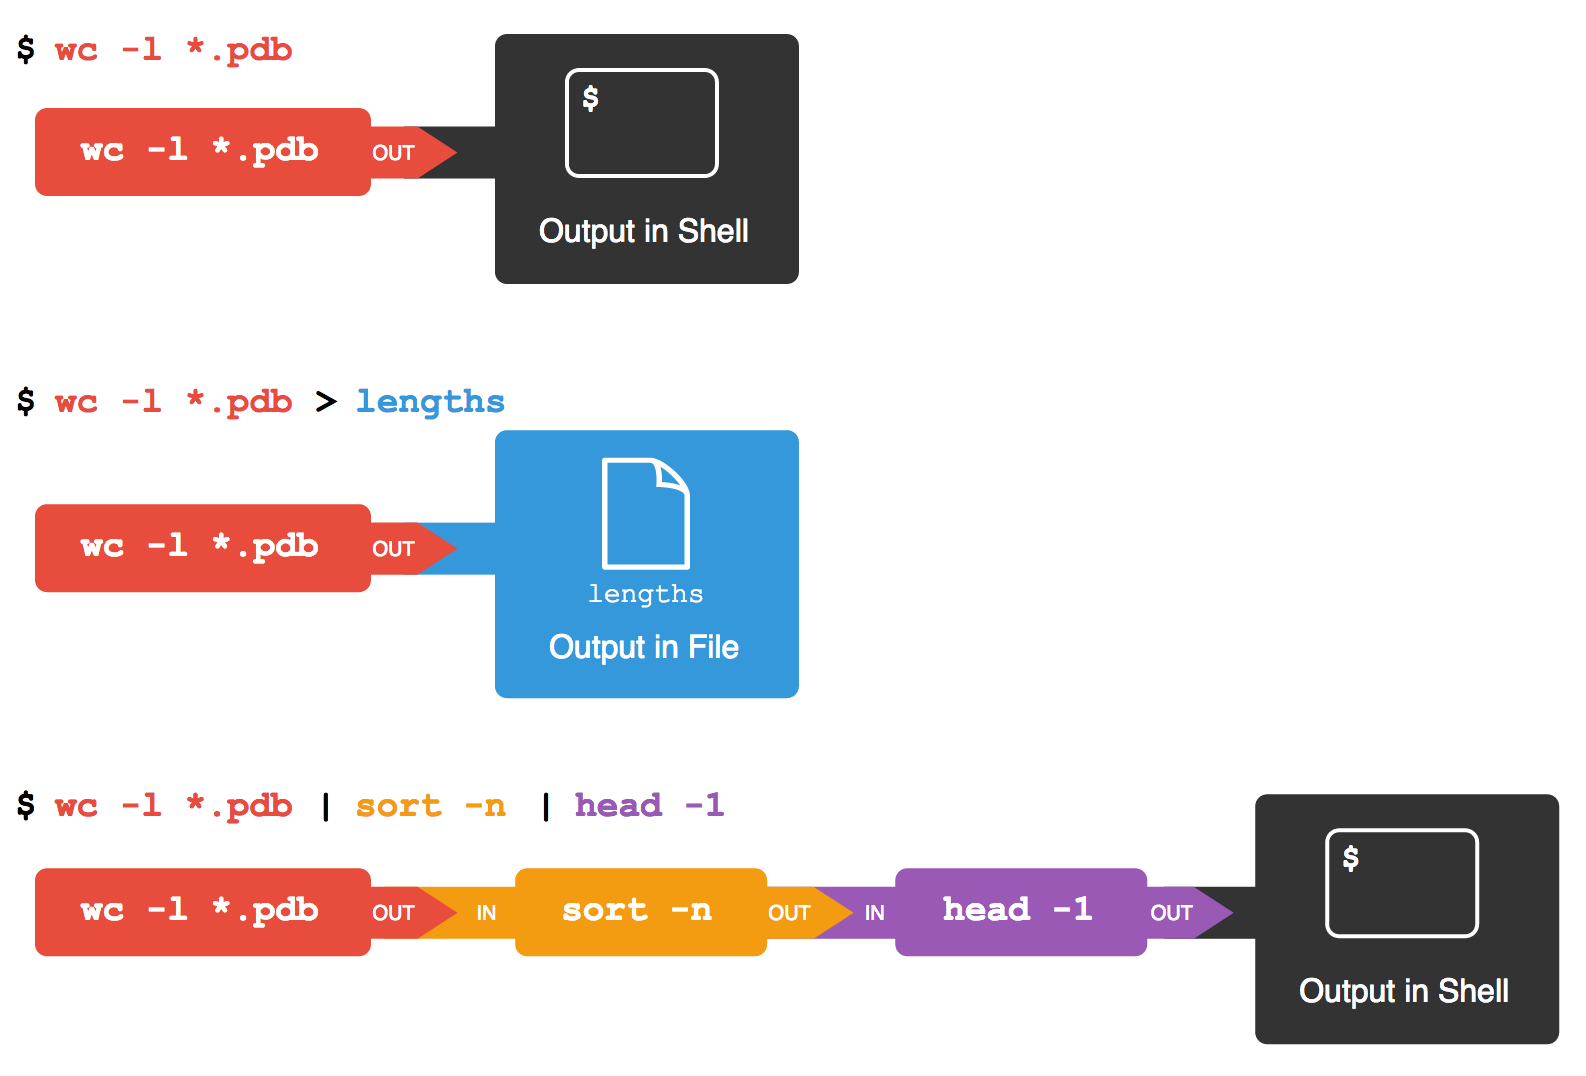
\includegraphics[width=0.7 \textwidth]{UnixPipe_flow.png}
	\caption{Minh họa về Pipe và Redirect trong Command Line}
	\label{fig:pipe_workflow}
\end{figure}

Cuối cùng, để kết hợp nhiều lệnh với nhau thành 1 pipe, mình dùng \texttt{|} để nối đầu ra của lệnh trước \texttt{wc -l *.pdb} tới đầu vào của lệnh sau là \texttt{sort -n} trong đó \texttt{-n} là 1 flag thông báo sort theo thứ tự số nhỏ tới lớn thay vì chữ từ a-z.
Vậy "\texttt{wc -l *.pdb | sort -n}" nghĩa là đếm mọi số dòng trong mọi file có đuôi \texttt{.pdb} rồi sort theo dòng từ nhỏ tới lớn. Cuối cùng mình sử dụng \texttt{head -1} để lấy file có số dòng nhỏ nhất.

\subsubsection{Ví dụ các bước xây dựng flow hoạt động của 1 Pipeline đơn giản}
\textbf{Ví dụ 1: Pipe đơn giản – lọc dữ liệu}
Giả sử bạn có file \texttt{users.csv} chứa danh sách người dùng, bạn muốn lọc ra các dòng chứa từ "admin".
\begin{verbatim}
cat users.csv | grep "admin"
\end{verbatim}

\textbf{Giải thích:}
\begin{itemize}
	\item \texttt{cat users.csv}: đọc toàn bộ nội dung file.
	\item \texttt{grep "admin"}: lọc các dòng có chứa từ "admin".
	\item \texttt{|}: kết nối hai lệnh – nội dung từ \texttt{cat} được chuyển cho \texttt{grep}.
\end{itemize}

\subsubsection*{Ví dụ 2: Redirect – ghi kết quả vào file}

Bây giờ bạn muốn lưu kết quả lọc trên vào file \texttt{admins.txt}:

\begin{verbatim}
cat users.csv | grep "admin" > admins.txt
\end{verbatim}

\textbf{Giải thích:}
\begin{itemize}
	\item \texttt{>} redirect output sang file mới tên là \texttt{admins.txt}.
	\item Nếu file đã tồn tại, nó sẽ bị ghi đè.
\end{itemize}

\subsubsection*{Ví dụ 3: Kết hợp pipe và append}

Lưu tiếp kết quả các dòng chứa “moderator” vào cùng file:

\begin{verbatim}
cat users.csv | grep "moderator" >> admins.txt
\end{verbatim}

\textbf{Giải thích:}
\begin{itemize}
	\item \texttt{>>} thêm nội dung vào cuối file \texttt{admins.txt}, không ghi đè.
\end{itemize}

\subsubsection*{Tóm tắt}

Pipe và redirect giúp bạn kết nối các công cụ nhỏ để xử lý dữ liệu một cách linh hoạt, ví dụ như:

\begin{verbatim}
cat data.csv | grep "2024" | cut -d',' -f1 | sort | uniq > results.txt
\end{verbatim}

Câu lệnh trên trích xuất cột 1 từ các dòng chứa "2024", sắp xếp và lọc trùng, sau đó ghi vào file \texttt{results.txt}.

% Part 2
\subsection{Filter Commands cho Data – Bộ lọc mạnh mẽ của Command Line}

Command Line trong Unix/Linux cung cấp các công cụ xử lý văn bản cực kỳ mạnh mẽ như \texttt{sed}, \texttt{awk}, \texttt{cut}, \texttt{tr}, và \texttt{grep}. Đây là các lệnh thường dùng để lọc, chỉnh sửa và trích xuất thông tin từ dữ liệu dạng văn bản (logs, CSV, JSON, v.v.). Mình có thể hình dung cách sử dụng cơ bản của từng lệnh với các ví dụ đơn giản sau:
\vspace{0.5em}
\subsubsection*{1. \texttt{grep} – Tìm dòng chứa mẫu (pattern)}
\begin{verbatim}
grep "ERROR" logfile.txt
\end{verbatim}
Tìm tất cả các dòng trong file \texttt{logfile.txt} có chứa từ \texttt{ERROR}.

\vspace{0.5em}
\subsubsection*{2. \texttt{cut} – Cắt cột hoặc ký tự trong dòng}
\begin{verbatim}
cut -d',' -f1,3 data.csv
\end{verbatim}
Trích xuất cột 1 và 3 (phân tách bằng dấu phẩy) từ file CSV.

\vspace{0.5em}
\subsubsection*{3. \texttt{awk} – Xử lý theo dòng và cột như một mini-script}
\begin{verbatim}
awk '{print $2}' users.txt
\end{verbatim}
In cột thứ hai trong mỗi dòng của file \texttt{users.txt} (dấu cách là mặc định).

\vspace{0.5em}
\subsubsection*{4. \texttt{sed} – Tìm và thay thế văn bản}
\begin{verbatim}
sed 's/admin/user/g' accounts.txt
\end{verbatim}
Thay mọi từ "admin" thành "user" trong file \texttt{accounts.txt} và in ra kết quả.

\vspace{0.5em}
\subsubsection*{5. \texttt{tr} – Chuyển đổi ký tự}
\begin{verbatim}
tr 'a-z' 'A-Z' < names.txt
\end{verbatim}
Chuyển toàn bộ chữ thường thành chữ in hoa trong file \texttt{names.txt}.

\vspace{1em}
\noindent
\textbf{Mở rộng:}
Các công cụ trên có thể kết hợp với nhau qua \texttt{pipe (|)} để xây dựng quy trình xử lý dữ liệu phức tạp. Hãy thử kết hợp chúng để:
\begin{itemize}
  \item Lọc các dòng có năm 2023 trong file logs.
  \item Trích cột thứ ba và chuyển thành chữ in hoa.
  \item Tự động thay thế định dạng ngày từ DD/MM/YYYY sang YYYY-MM-DD.
\end{itemize}


\subsection{Trích xuất dữ liệu từ files lớn}

\subsection{Xử lý dữ liệu JSON với jq}

\subsubsection{Xử lý dữ liệu JSON với jq phần 1}

\subsubsection{Xử lý dữ liệu JSON với jq phần 2}


\subsection{Xử lý CSV qua command line}


\subsection{Phân tích logs với command line}


\subsection{Kết hợp các commands phức tạp}


\subsection{xargs - xử lý dữ liệu song song}

\subsection{Xử lý dữ liệu thực tế}

\subsection{Tải dữ liệu từ internet (wget, curl)}

\subsection{Làm việc với files né}

\subsection{giải nén và xử lý nhiều files}

\subsection{Bài tập thực hành}

\begin{enumerate}
	\item \textbf{Xử lý file CSV người dùng}\\
	Xử lý \texttt{users\_2023-01-01.csv}: Đếm người dùng theo khu vực. Lọc người dùng theo trạng thái ``Active''. Sắp xếp theo tần suất truy cập (giảm dần).

	\item \textbf{Phân tích dữ liệu JSON thời tiết}\\
	Phân tích file \texttt{weather\_hanoi.json}. Trích xuất nhiệt độ, độ ẩm theo ngày. Tính nhiệt độ và độ ẩm trung bình.

	\item \textbf{Tạo báo cáo hiệu suất mô hình}\\
	Phân tích file \texttt{model\_logs.txt} để tổng hợp precision, recall theo ngày và phát hiện xu hướng suy giảm (đếm số ngày có precision $<$ 0.75 và recall $<$ 0.75).

	\item \textbf{Tự động hóa quy trình báo cáo}
	\begin{itemize}
		\item Tạo thư mục \texttt{project/reports}.
		\item Kết hợp các lệnh, lưu kết quả vào \texttt{project/reports/weekly.txt}.
		\item Tạo file dữ liệu (\texttt{region\_counts.dat}) cho biểu đồ.
		\item Dùng \texttt{gnuplot} vẽ biểu đồ người dùng theo khu vực (\texttt{users\_by\_region.png}).
	\end{itemize}
\end{enumerate}

\subsection{Tóm tắt và Tổng kết phần 3}

\end{document}
